\chapter[Analysis and Results]{Analysis and Results}
\label{ch:result}
The following chapter contains the analysis of the data presented in chapter \ref{ch:data}. First is the analysis of the two computer generated synthetic data, before the methods are applied to the real life commodity data.\\

For the POT MCMC method, as described in chapter \ref{ch:ama}, the optimal acceptance rate for a single dimensional normal target distribution is $44\%$ while it is $23.4\%$ for higher dimensional multivariate normal target distribution. The parameters $\xi$ and $\phi$ probably does not follow a bivariate normal target distribution, and they are only two dimensional, hence the optimal acceptance rate is unknown. Calculating the effective sample size for multiple different MCMC simulations on different data sets, using a variety of acceptance rate between $20\%$ and $50\%$, shows a trend suggesting $30\% \leq a \leq40\%$. For the rest of this work $a$ is set to $0.35$, which will converge the AMCMC towards an acceptance rate of $35\%$, by the theory described in chapter \ref{ch:ama}.

\section{Analysis of Syntetic data}
The goal of this section is to use the ACER and POT MCMC method to analyze controlled data for better conformation of prediction and test reliability. The Pareto distribution is i.i.d. while the simulated \textcolor{red}{AR(1)-APARCH(1,1)?}, is not. It is also interesting to study the performance difference for the two method in each cases.
\subsection{Pareto Distirbution}
One of the advantage of analyzing the Pareto distributions, is that the theoretical distribution is known, hence the exact analytical values can be achieved even for extreme cases. For testing, the yearly, decadal, centennial and millennial event or in probability $1/365$, $1/3650$, $1/36500$ and $1/3650000$ respectively, are estimated and compared with the exact values.

Given the definition of VaR equation \eqref{eq:vardef}, the exact VaR for the Pareto distribution can be found by 
\begin{equation*}
\text{VaR}_\alpha=\frac{1}{\alpha^{1/\beta}}.
\end{equation*} 
For the estimated prediction interval, the exact probability for a future $n$th maximum to arriving whiten that limit is developed by combining equation \eqref{eq:basicextreemiid} and \eqref{eq:paretocdf}, which result in \begin{equation*}
\Pr \left( m_n^{(-)} \leq M_n \leq m_n^{(+)} \right)=\left( 1-{ m_n^{(+)}}^{-\beta} \right)^n - \left( 1-{ m_n^{(-)}}^{-\beta} \right)^n,
\end{equation*}
where $m_n^{(+)}$ and $m_n^{(-)}$ is the upper and lower limits respectively.

The Pareto data from figure \ref{fig:paretodata}, with $\beta=3$ is analyzed for a walkthrough of how the methods are used, and result interpretation. The exact VaR for each case are represented in table \ref{table:paretovar}.

\begin{table}[h]
\centering
\begin{tabular}{ l c r}
  Event & $\alpha$ & $\text{VaR}_\alpha$  \\
  \hline
  Yearly & 1/365 & 7.147 \\
  Decadal & 1/3650 & 15.397\\
  Centennial & 1/36500 & 33.171\\
  Millennial & 1/365000 & 71.466\\
\end{tabular}
\caption{The exact VaR for each event with the corresponding probability $\alpha$, for the Pareto distribution with $\beta=3$.}
\label{table:paretovar}
\end{table}

Since the data are i.i.d., the ACER methods will use $k=1$, and the POT MCMC method will not need any decluttering or threshold analysis. In theory the point for where regular tail behavior starts for the ACER method, and the threshold for the MCMC method could be selected to $1$, which would make use of the entire data set without removing lower data. In real life such a situation is unrealistically, thus both is selected to $1.5$. Consequently, out of the total $9 \ 125$ Pareto distributed points, $2 \ 728$ exceeds $1.5$ and is used for future analysis.

The POT MCMC method is set to generate $100 \ 000$ realizations. In figure \ref{fig:paretoconvergence} the first $1 \ 000$ realizations is shown with starting conditions $[\xi^0,\phi^0]=[1,1]$. The plot converges within a few numbers of steps, while the variance of the points is adapting for some more iterations. Points generated after convergence, does follow the correct distribution, the variance only affects the effective sample size, even though it has not settled in yet. Data between $1$st and $500$th realization is selected as burn-in and is discarded for later analysis, resulting in an effective sample size of $13 \ 580$ for $\xi$ and $14 \ 746$ for $\sigma$. %The acceptance rate was $38\%$, which is reasonable close to the preset value of $a=0.35$. The deviation is a result of the adaptive steps.
\begin{figure}
  \centering
    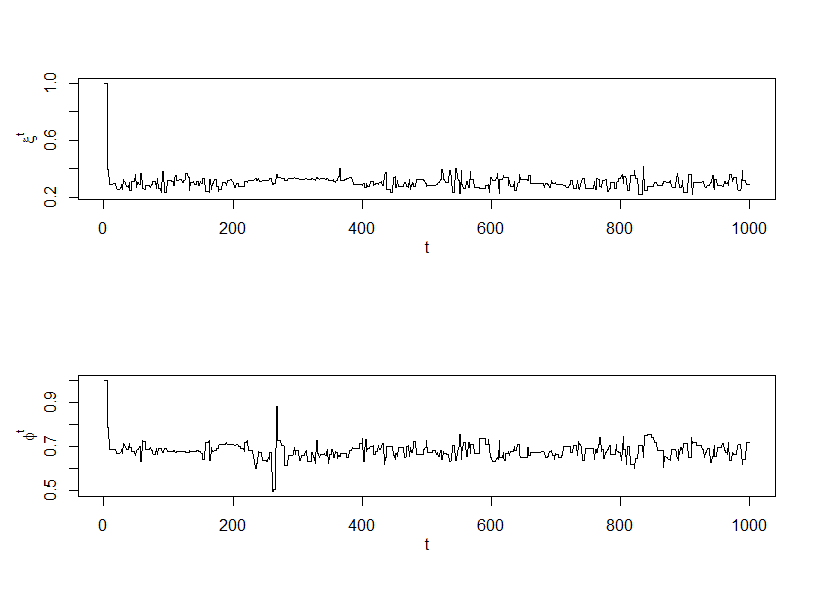
\includegraphics[width=1\textwidth]{fig/result/paretoconvergence.png}
  \caption{The first $1 \ 000$ realizations of the POT MCMC method for $\xi$ and $\phi$.}
  \label{fig:paretoconvergence}
\end{figure}
The realized distribution of $\xi$, $\sigma$ and $\beta$ for the POT MCMC method can be seen in figure \ref{fig:paretoxisigmabeta}
\begin{figure}
  \centering
    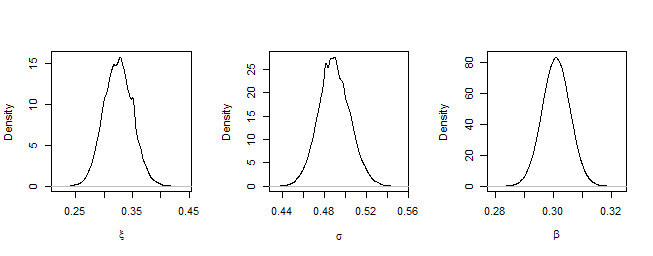
\includegraphics[width=1\textwidth]{fig/result/paretoxisigmabeta.png}
  \caption{The estimated posterior density of the POT MCMC parameters $\xi$, $\sigma$ and $\beta$.}
  \label{fig:paretoxisigmabeta}
\end{figure}

For the ACER method, the estimates, together with the upper and lower confidence limits can be seen in table \ref{table:paretoacerest}, with corresponding lines plotted in figure \ref{fig:paretoacermcmc}.
\begin{table}[h]
\centering
\begin{tabular}{ l c c c c r}
    & $a$ & $b$ &$c$ & $q$ & $\xi$  \\
  \hline
  Upper $95\%$ CI line& $2.824$ & $1.029$ & $1.626$ & $0.577$ & $0.769$ \\
  Estimated line& $2.756$ & $1.000$&$1.356$&$0.690$&$0.545$\\
  Lower $95\%$ CI lien & $3.105$ & $1.000$&$0.652$&$1.747$&$0.110$\\
\end{tabular}
\caption{The estimated ACER parameters together with the upper and lower $95\%$ confidence interval line parameters. }
\label{table:paretoacerest}
\end{table}

Comparison of the ACER and POT MCMC estimated probability functions with the real Pareto distribution can be seen in figure \ref{fig:paretoacermcmc}. Defining loss as an increase in value, the plot can also be interpreted as $\alpha$ against $VaR_\alpha$.
It is noted that the estimates for the POT MCMC are closer to the real distribution, with slimmer confidence interval. It is not surprisingly that the POT MCMC method perform better than the ACER method, since the points are i.i.d. The ACER methods capability of capturing data dependency is not necessary for the Pareto distribution, while the POT MCMC method uses an unrealistically large dataset for estimation.
\begin{figure}
  \centering
    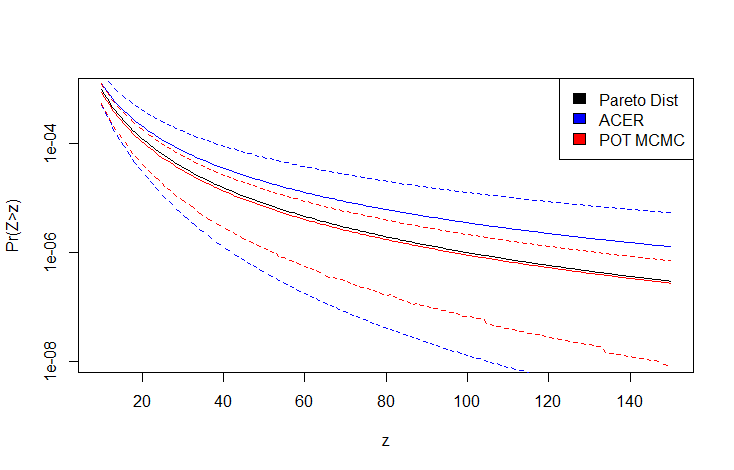
\includegraphics[width=1\textwidth]{fig/result/paretoacermcmc.png}
  \caption{A plot visualizing the estimated ACER and POT MCMC probabilities, together with the exact Pareto distribution. The estimates are shown in solid lines while the upper and lower $95\%$ confidence and credible limits are dashed.}
  \label{fig:paretoacermcmc}
\end{figure}

Using the theory from chapter \ref{ch:predconf}, the distribution of the maximum event for the upcoming year, decade, century and millennium is prediction for the two methods. Figure \ref{fig:paretopred} shows the distribution of the exact Pareto prediction together with the estimated ACER and POT MCMC, with prediction intervals.
\begin{figure}
  \centering
    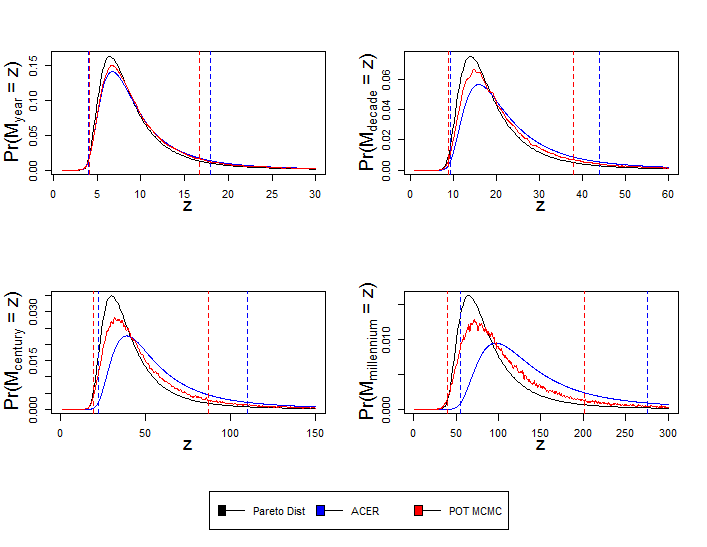
\includegraphics[width=1\textwidth]{fig/result/paretopred.png}
  \caption{The estimated ACER and POT MCMC future year, decade, century and millennium predicted probability functions together with the true distribution. Solid line shows the probability distribution functions while dashed lines mark each methods corresponding $90\%$ prediction interval.}
  \label{fig:paretopred}
\end{figure}

An approach for validating the methods prediction interval, can come from calculating how much of the real distribution was contained within the predicted intervals. See table \ref{table:paretopred} for the corresponding values. 
\begin{table}[h]
\centering
\begin{tabular}{ l c c c r}
    & year & decade &century & millennium \\
  \hline
  ACER& $93.5\% \ (13.9)$ & $94.8\% \ (34.8)$ & $93.6\% \ (87.58)$ & $87.1\% \ (220.9)$  \\
  POT MCMC& $92.0\% \ (12.7)$&$92.8\% \ (28.9)$&$94.1\% \ (67.6)$&$95.4\% \ (159.9)$ \\
\end{tabular}
\caption{The amount of the exact distribution contained in the predicted $90\%$ interval, with interval length in brackets, for the ACER and POT MCMC method.}
\label{table:paretopred}
\end{table}
The table shows that both methods in each case predict reasonable close to $90\%$ interval, while the POT MCMC method consistently perform better with respect to interval width.

By regenerating $30$, Pareto distribution $9 \ 125$ points series, using a random $\beta$ between $1$ and $5$ for each, the investigation above can be scaled up for a more accurate analysis. 

DEFINER VARDIER SOM $\mu_{\hat{VaR}-VaR}$ OSV, KALK FOR MANGE, LAG TABELL SOM PAA TAVLEN!

 

\subsection{Commodity Generated Data}

\section{Commodity Data}